\documentclass[18pt]{beamer}
\usepackage[utf8]{inputenc}
\usepackage{templates/mytemplate}
\usepackage{templates/beamerthemekit}
\usepackage{graphicx}
\usepackage{microtype}
\usepackage{listings}
\usepackage{hyperref}
\usepackage{multicol}

%% SLIDE FORMAT

\usepackage{amssymb}

\title{First look at Cosmic CDC Tracks and Ideas for Estimating the Finding Efficiency} 
\subtitle{F2F Tracking Meeting}
\author{\underline{Michael Eliachevitch}}
\date{18 September 2018}
\titleimage{kitlogo_en_rgb}
\institute{ETP - KIT}

\begin{document}

  \selectlanguage{english}

  \begin{frame}
  \titlepage
  \end{frame}

  \begin{frame}
    \frametitle{Introduction}
    \begin{itemize}
    \item Currently tracking validation is done in MC by comparing found tracks vs. tracks from MC truth
    \item First data from Global Cosmic Run 2017 is in. Can we use it? 
    \end{itemize}
  \end{frame}

  \begin{frame}
    \frametitle{GCR Data and MC}
    \begin{itemize}
    \item use data from Global Cosmic Run (GCR) taken in July 2017
    \item use run numbers 3100--3370 (sugggested by Dong Thang)
      $\Rightarrow$ total 2.8 Million cosmic events with trigger selecting central tracks\\
    \item also produced 50 Million cosmic MC events with GCR setup
      \begin{itemize}
      \item same as official MC group: large ``accept box'' of 8\,m $\times$ 8\,m $\times$ 8\,m 
      \item no triggger in simulation, do kinematic cuts on central region ($d_0, z_0$)\\
        $\Rightarrow$  $\sim$10 times less statistics than in data remain
      \end{itemize}
    % \item Links to information on data and MC production
    %   \begin{itemize}
    %   \item Data production: \footnotesize{\url{https://confluence.desy.de/display/BI/Data+Production+Global+Cosmics+Run+Data\#DataProductionGlobalCosmicsRunData-Runinfo}}
    %   \item MC production: \footnotesize{\url{https://confluence.desy.de/display/BI/Data+Production+Global+Cosmics+Run+MC}}
    %   \end{itemize}
    \end{itemize}

    \begin{block}{Links to information on data and MC production}
      \begin{itemize}
      \item Data: \footnotesize{\url{https://confluence.desy.de/display/BI/Data+Production+Global+Cosmics+Run+Data\#DataProductionGlobalCosmicsRunData-Runinfo}}
      \item MC: \footnotesize{\url{https://confluence.desy.de/display/BI/Data+Production+Global+Cosmics+Run+MC}}
      \end{itemize}
    \end{block}
  \end{frame}

  \begin{frame}
    \frametitle{Look at Kinematic Distributions:\\Data with trigger and MC}
    \begin{itemize}
    \item left data (includes triggerr), right MC (without trigger)
    \item use (preliminary) cuts for selection of central tracks (red lines)
    \item B-Field mapper not in simulation
    \end{itemize}
    \begin{center}
      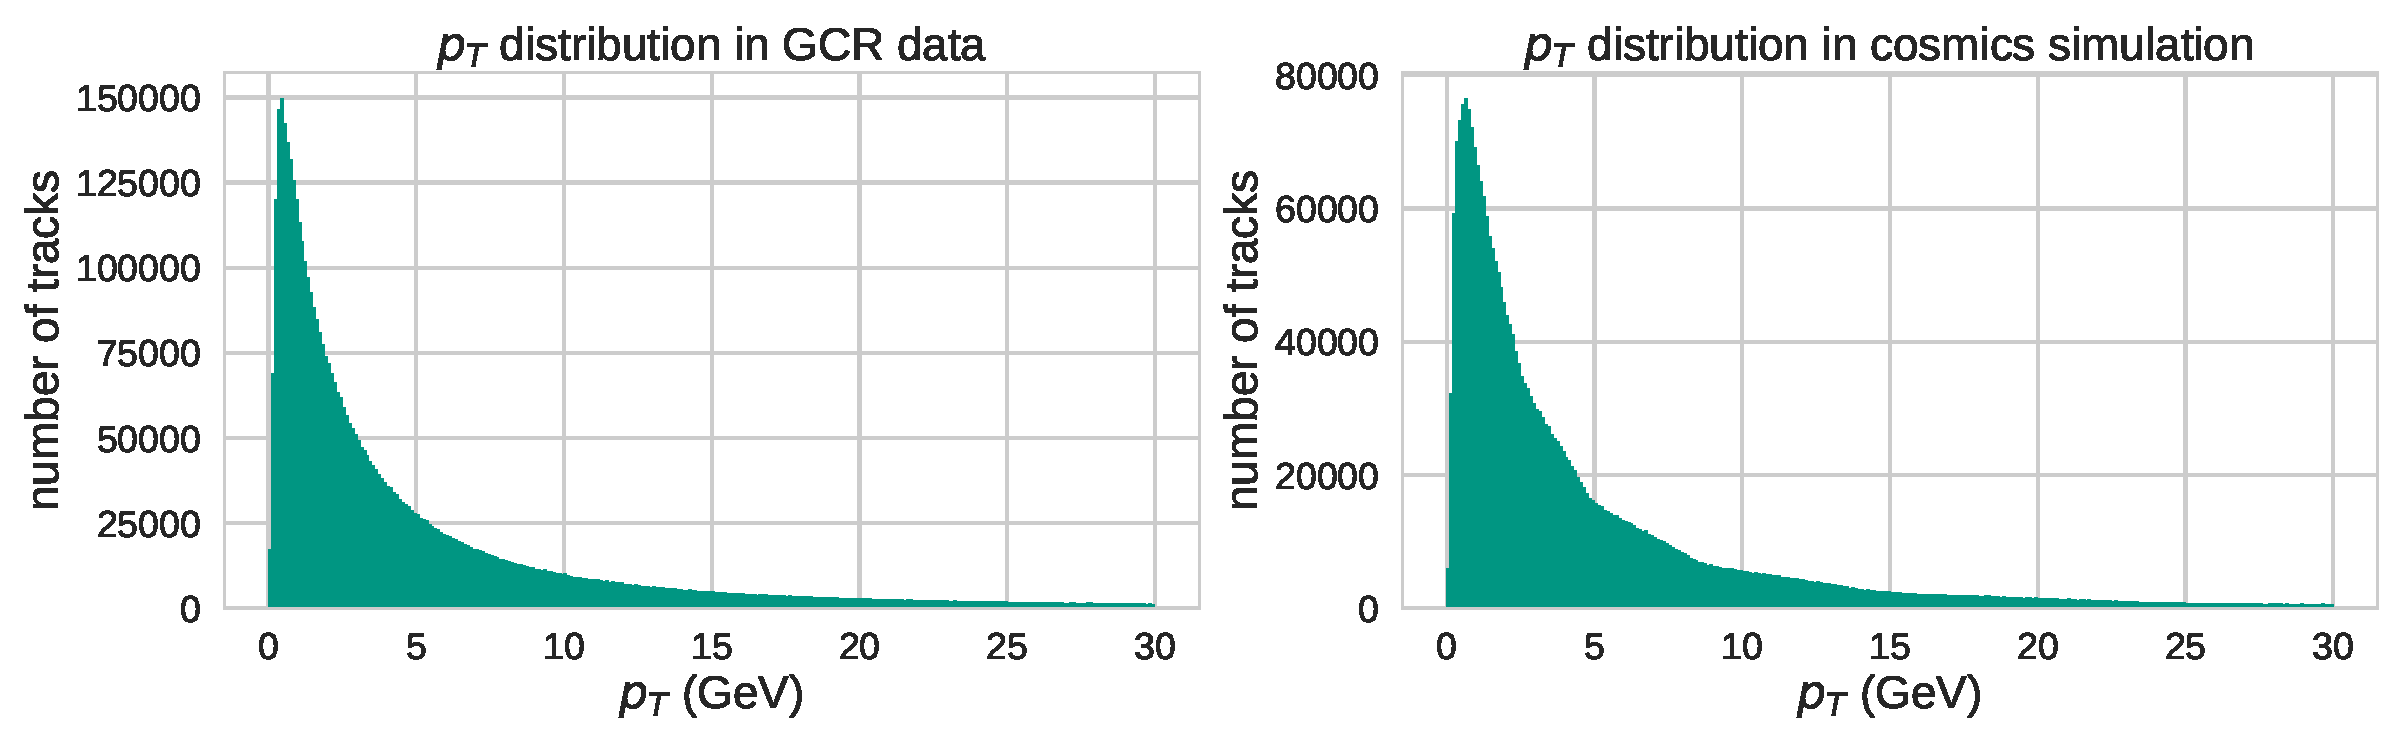
\includegraphics[width=0.65\textwidth]{figures/distributions/gcr_pt_distribution_uncut.pdf}\\
      \includegraphics[width=0.65\textwidth]{figures/distributions/gcr_omega_distribution_uncut.pdf}
    \end{center}
    \begin{itemize}
    \item $p_T$ distributions seem similar, but more events with $\omega = 0$
    \end{itemize}
  \end{frame}

  \begin{frame}
    \begin{center}
      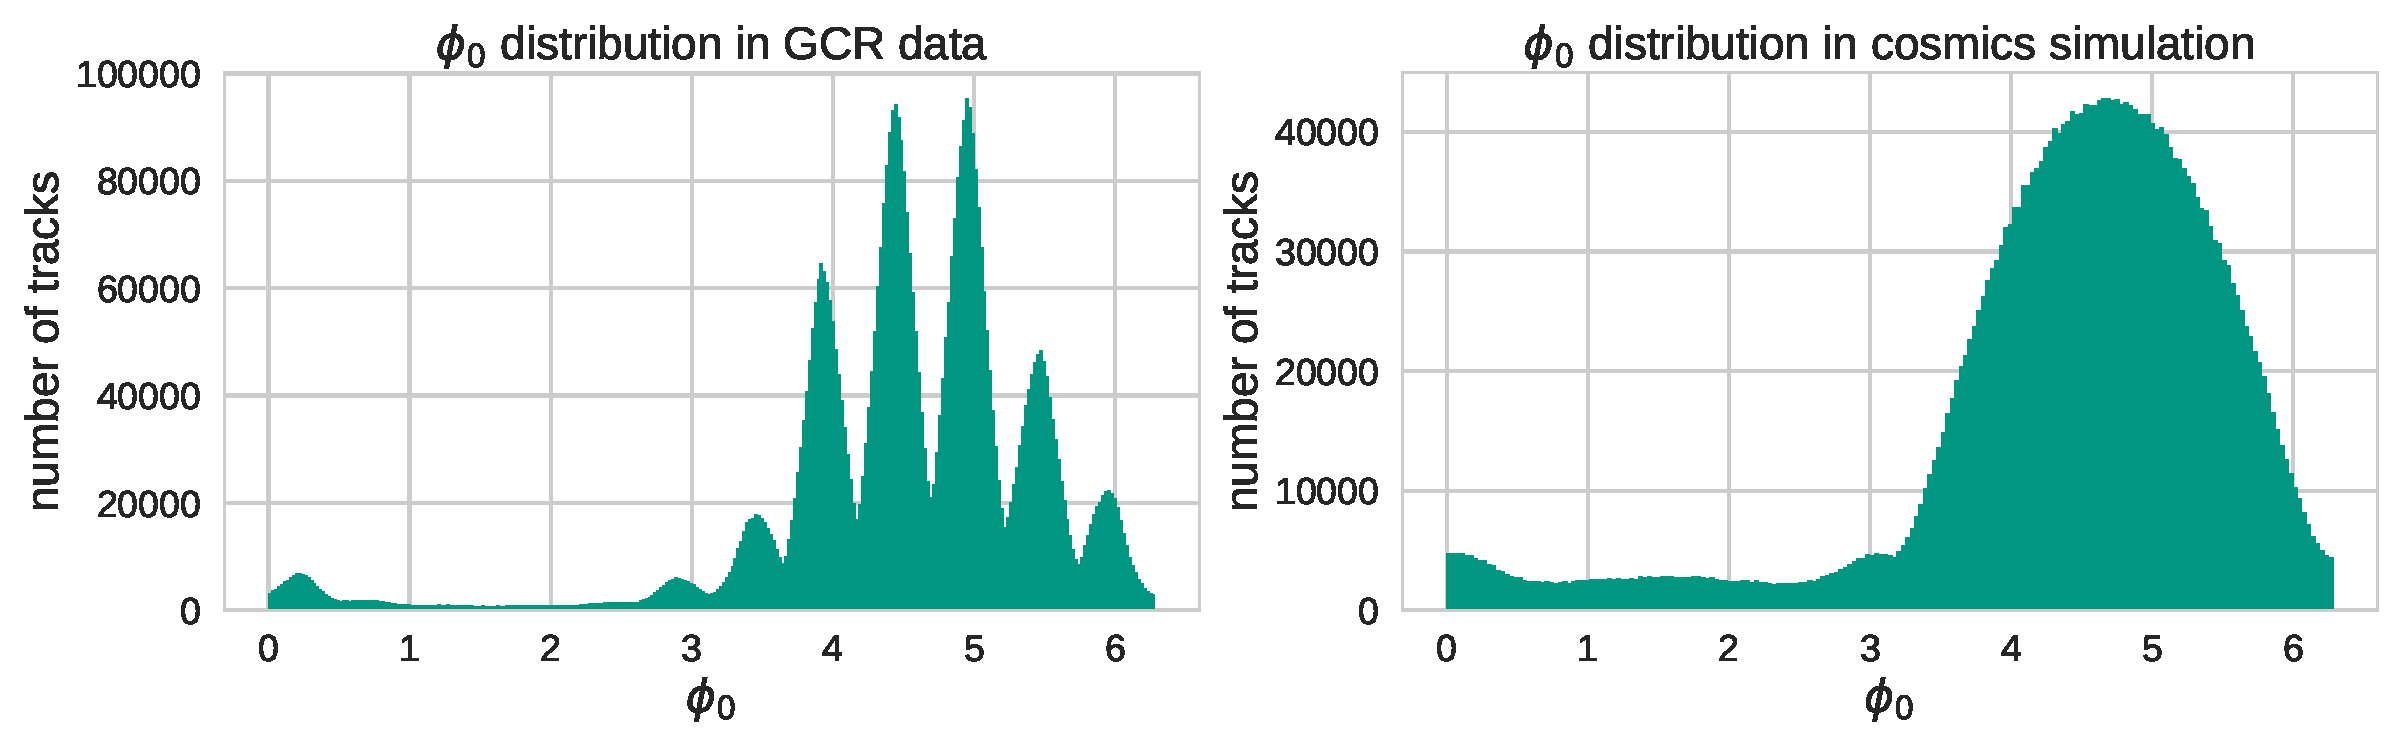
\includegraphics[width=0.65\textwidth]{figures/distributions/gcr_phi0_distribution_uncut.pdf}\\
      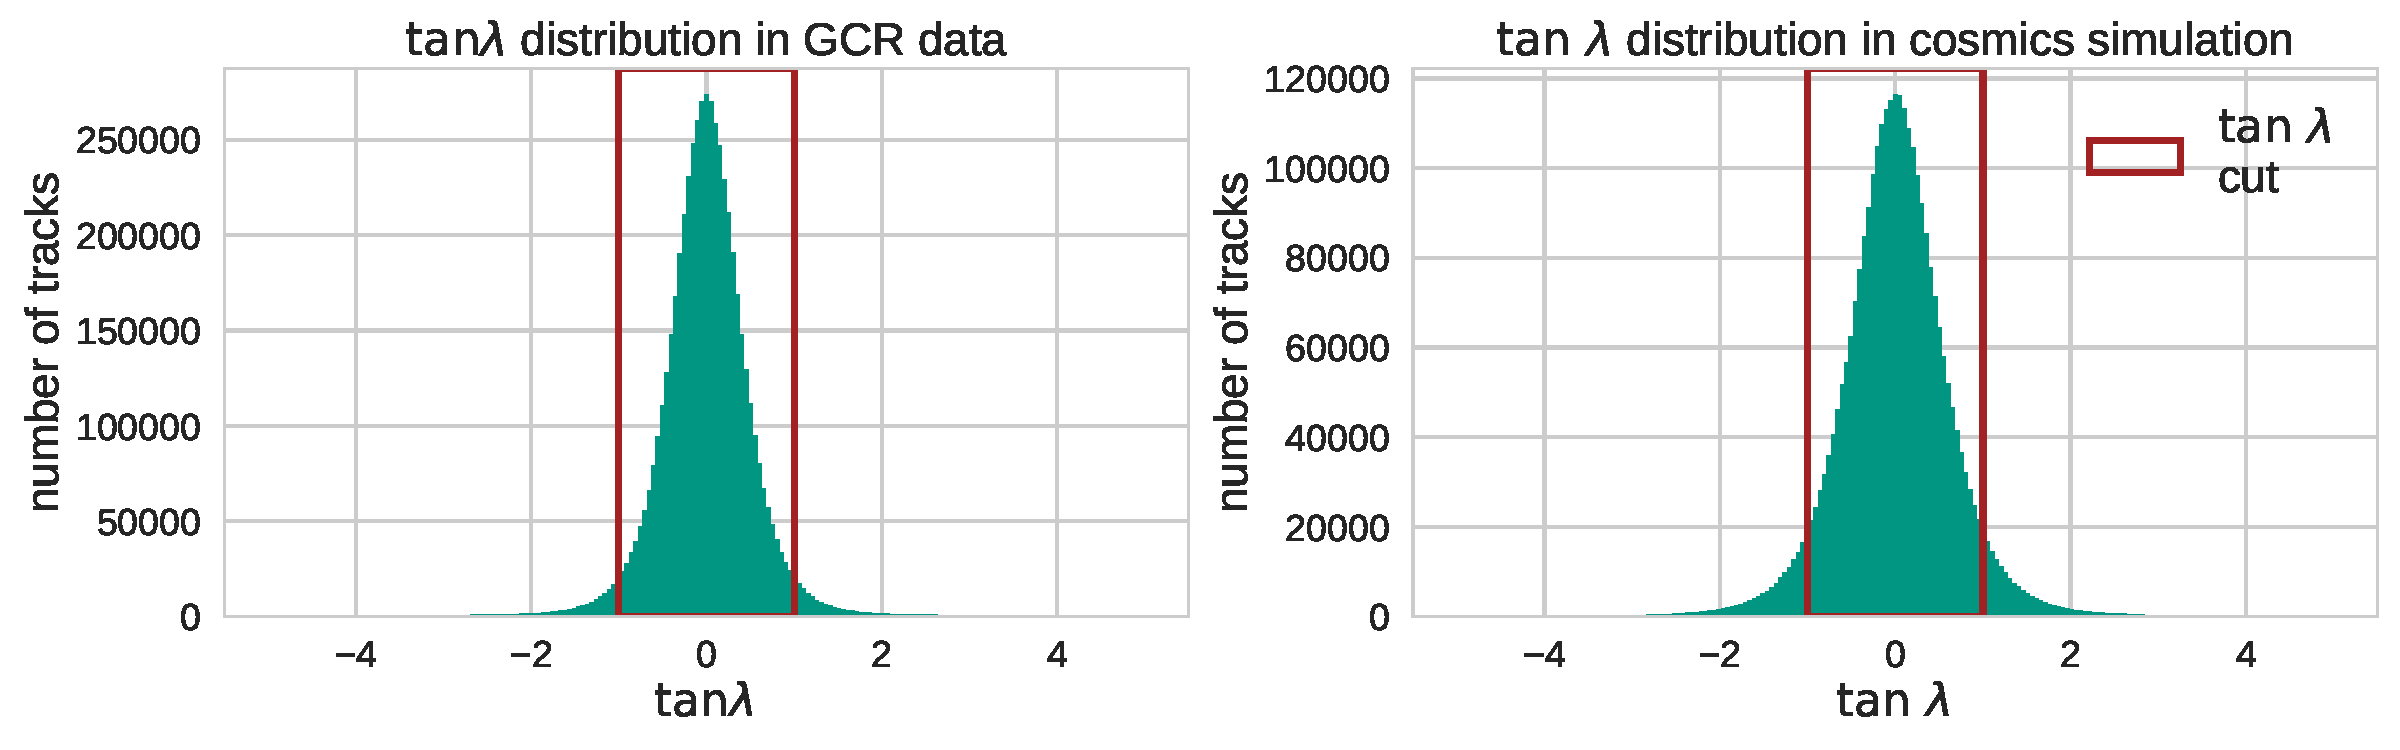
\includegraphics[width=0.65\textwidth]{figures/distributions/gcr_tan_lambda_distribution_uncut.pdf}
    \end{center}

    \begin{itemize}
    \item effects of B-field mapper visible in $phi_0$ distribution
    \end{itemize}
  \end{frame}

  \begin{frame}
    \begin{center}
      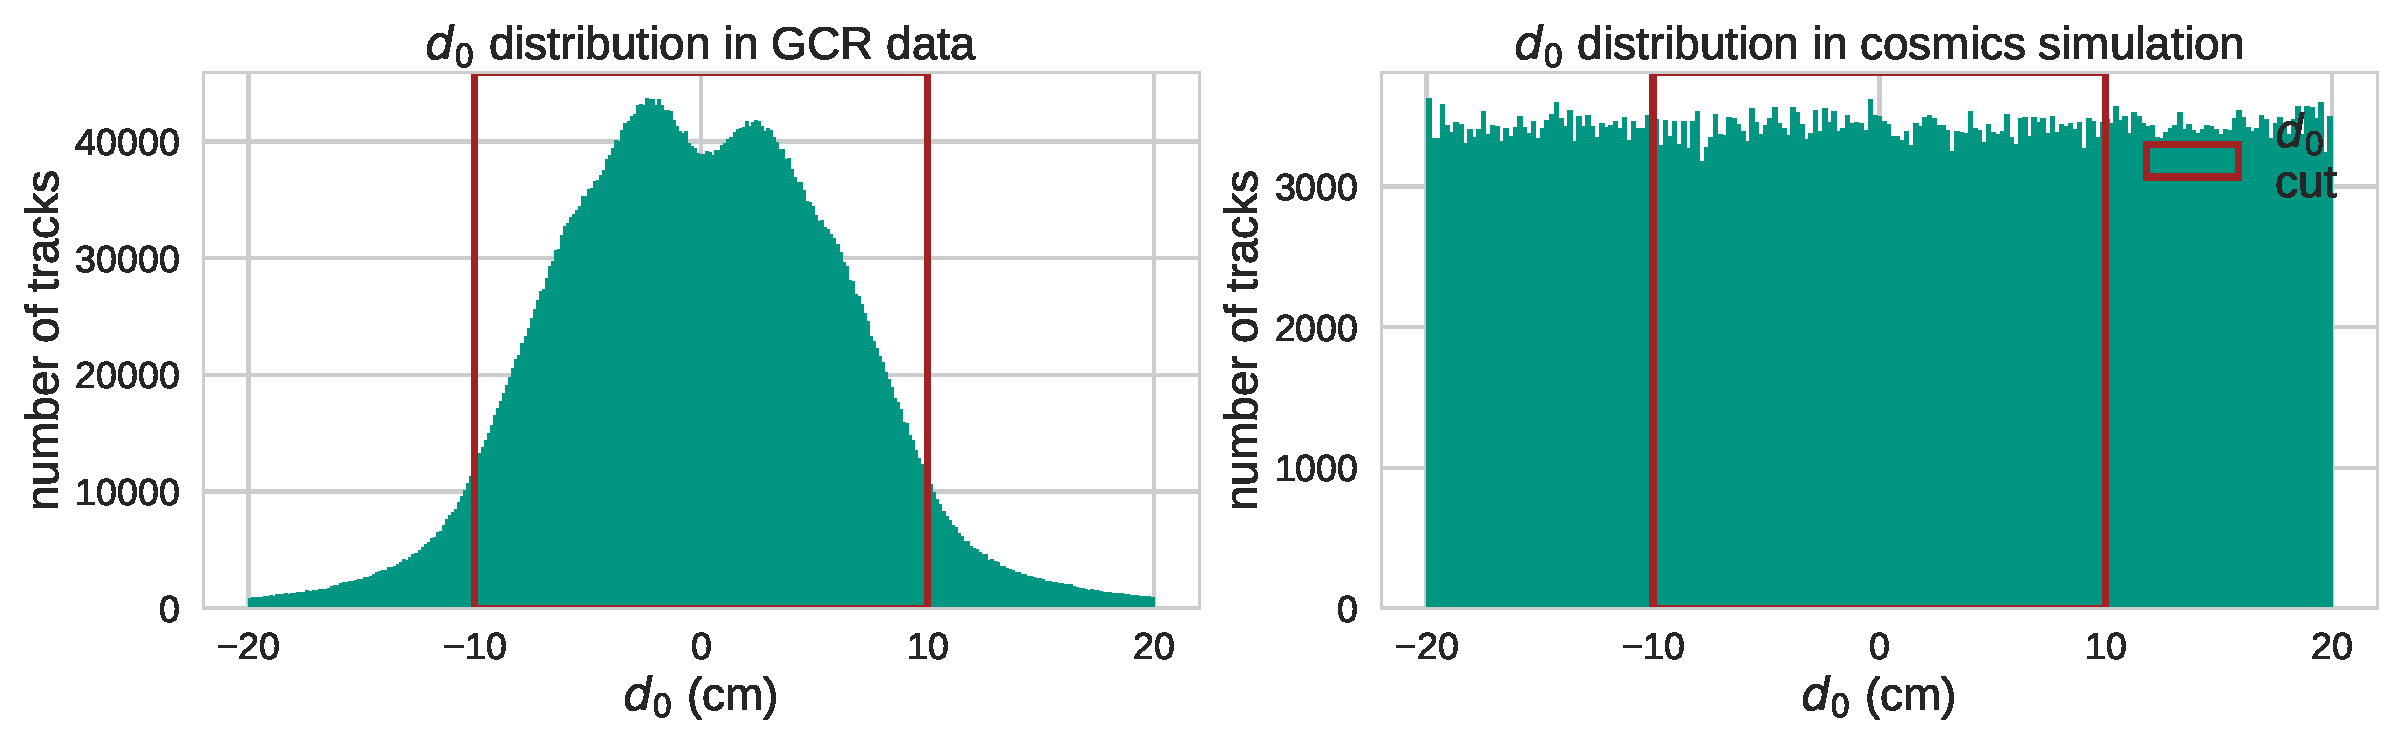
\includegraphics[width=0.65\textwidth]{figures/distributions/gcr_d0_distribution_uncut.pdf}\\
      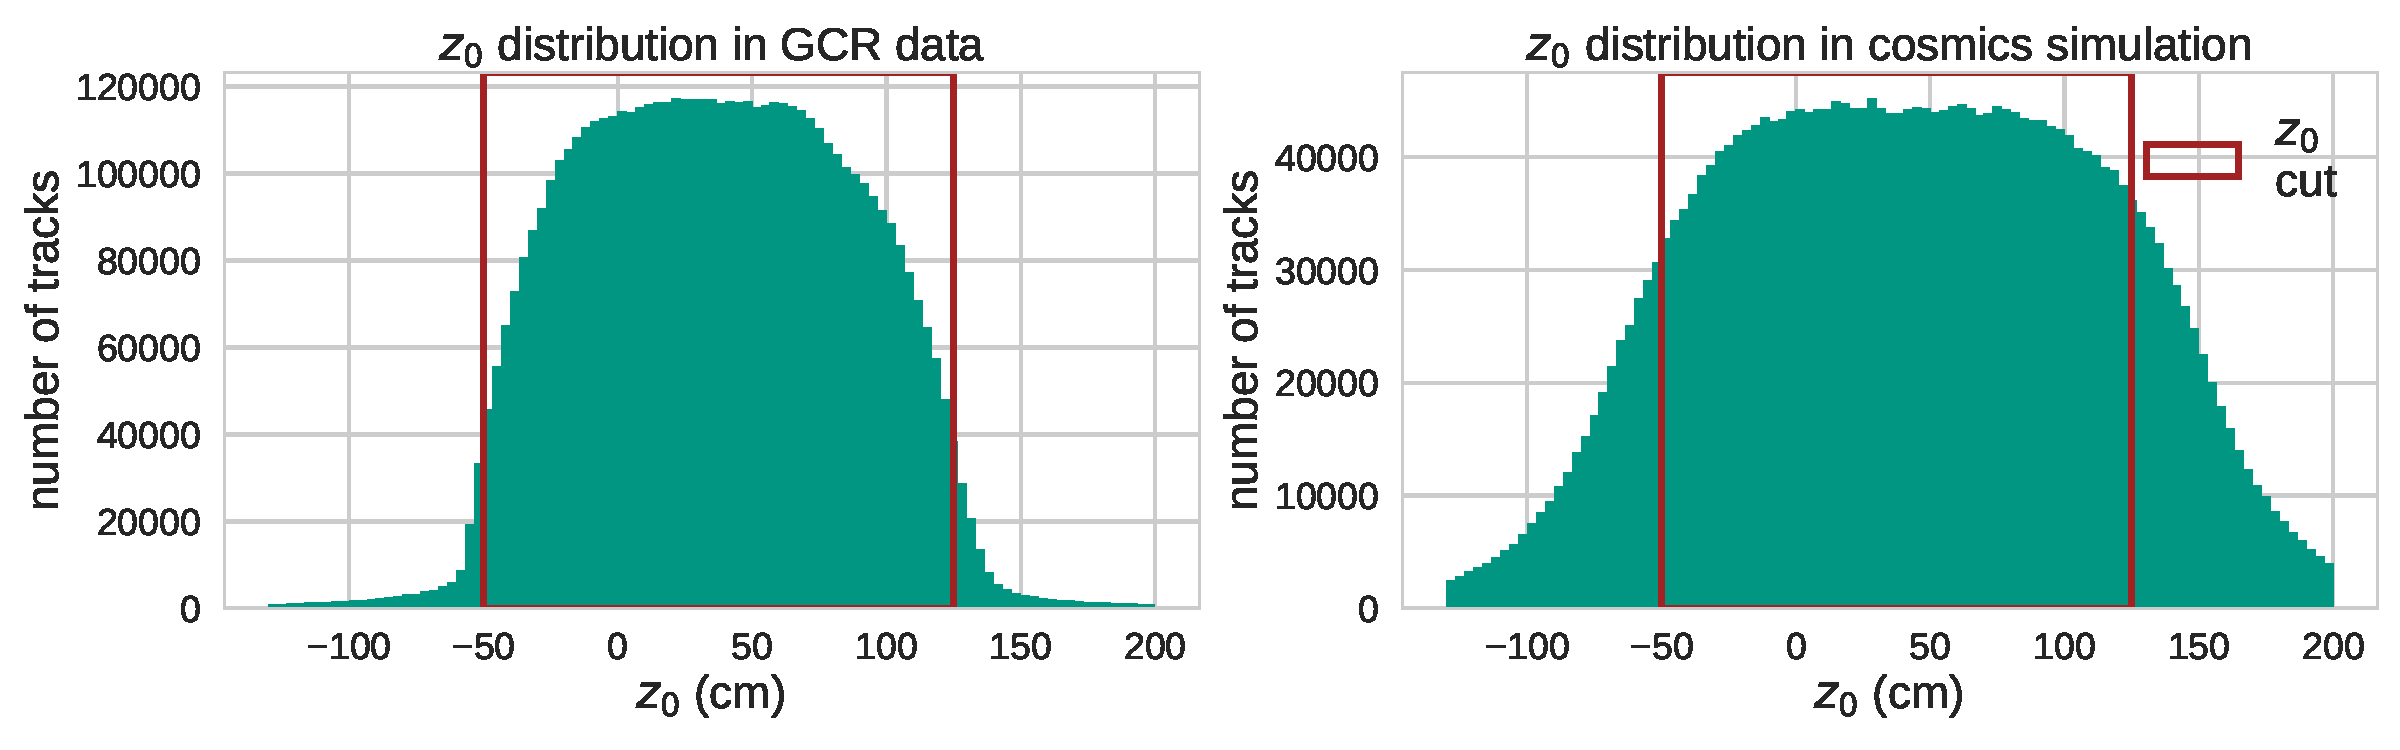
\includegraphics[width=0.65\textwidth]{figures/distributions/gcr_z0_distribution_uncut.pdf}
    \end{center}
    \begin{itemize}
    \item distribution in MC due to lack of trigger much wider, use cuts on central region
    \end{itemize}
  \end{frame}

  \begin{frame}
    \frametitle{Idea: Cosmics-Data based Estimation of Finding Efficiency}
    \begin{itemize}
    \item tracks passing through the centre (where SVD will be) are split
    \item usually reconstructed as two \texttt{NonMergedRecoTracks},
      which are then merged to \texttt{RecoTracks}
    \item get estimate of finding efficiency from events where two tracks expected, but only one found (finding fails)
    \item idea: compare results with MC based finding efficieny from \texttt{TrackMatchLookUp}
    \end{itemize}
    \pause
    \begin{block}{}
      \begin{equation*}
        \label{eq:cosmic_eff}
        \text{Finding efficiency} = \frac{N_\mathrm{2\ tracks\ found}}{N_\mathrm{2\ tracks\ expected}}
        = 1 - \frac{N_\mathrm{1\ track\ found}}{N_\mathrm{2\ tracks\ expected}}
      \end{equation*}             %
    \end{block}
    where $N_\mathrm{1\ track\ found}, N_\mathrm{2\ tracks\ found}, \in N_\mathrm{2\ tracks\ expected}$, so that $N_\mathrm{1\ track\ found} + N_\mathrm{2\ tracks\ found} = N_\mathrm{2\ tracks\ expected}$.
  \end{frame}

  \begin{frame}
    \frametitle{Selection of expected two-track events in MC and data}
    \begin{itemize}
    \item TODO
    \end{itemize}
  \end{frame}

  \begin{frame}    
    \frametitle{``Background'': Events where only one track is expected}
    
  \end{frame}

  \begin{frame}
    \frametitle{WIP: Select }
    
  \end{frame}

  \begin{frame}
    \frametitle{Testing the Method with Preliminary Cuts (not from MC)}
    \begin{itemize}
    \item 
    \end{itemize}
  \end{frame}

  
\end{document}

%%% Local Variables:
%%% mode: latex
%%% TeX-master: t
%%% End:
